\documentclass[11pt]{article}
\usepackage[margin=1in]{geometry}
\usepackage{graphicx}
\usepackage{wrapfig}
\usepackage{caption}
\usepackage{subcaption}


\begin{document}

\title{How does the CAL determine a direction?}
\author{}
\date{}
\maketitle

We thought it was a good idea to get these ideas and what I've learned about how the the CAL determines a direction down in the form a memo.  the basic structure is of this memo will be to first go how the CAL gets a direction and second how we have modified the direction analysis to be optimized for hadrons.  

\section{How the CAL gets a direction}
After digging around in the code there are appear to be two main methods in which the CAL finds a direction:
\begin{enumerate}
\item Directional Fitter
\item Moment Analysis
\end{enumerate}

Let's go over each method in detail.  

\subsection{Directional Fitter}

The directional fitter is a program that fits energy weighted centroid position in each layer to find the centroid and direction of incident particle.  

The first step is to find the energy weighted centroid in each layer of the CAL.  This is done with:

\begin{eqnarray}
\vec{p} = \frac{1}{E_{{tot}}} \sum_{i} \vec{x_i} E_i
\end{eqnarray}

Since the CAL is arranged in a hodoscopic array and the position is only measured along the long axis of crystal, each layer will only provide the x or y and z position of the centroid.  Now we have three global static quantities: m-fit-p-layer, m-fit-v-layer, and m-fit-errp-layer.  

m-fit-p-layer is the xyz position of the energy weighted centroid in each layer.  m-fit-v-layer is the vector pointed perpendicular to the direction of the crystal direction.  m-fit-errp-layer is the error which is the error in position measurement in each layer.  m-fit-errp-layer is found by the fraction of energy in said layer multiplied by the number of layers used to find the direction.  

We now want to find the line that minimizes the $\chi^2$.  We compute the $\chi^2$ by measuring the distance squared between the lines formed from the data and the fit.  To find the $\chi^2$ we take that distance squared and divide by the square of the number of layers used in the fitting analysis and multiply by m-fit-errp-layer.  

Finding the direction and centroid position has three steps.  First step is to coarsely map the entire parameter space with the only two free parameters being $\theta$ and $\phi$.  The centroid position is kept fixed during this step.  This does not actually minimize any value, we just wish to find the good starting positions for the Minuit fitter which we use in the next step.  Once we have found the general area where the $\chi^2$ is minimized we then use Minuit fitter and finer step sizes.  In this step we reduce the step size by a factor of ten and use the direction determined from the previous step as the initial direction.  The centroid position is still fixed in this step.  Using the results from the previous step the third and final step uses the Minuit fitter and has four free variables: $\theta$, $\phi$, xpos, and ypos.   Note that zpos is not fit and held fixed.  

The results of directional fitter is the direction and position of the centroid.  We use these results in the moment analysis.

\subsection{Moment Analysis}

The moment analysis is an iterative processes where the energy weighted position from each crystal is used to form an inertia tensor where one of the eigenvectors of this tensor represents the direction of the incoming particle.  

The zeroth step is to determine the location of the initial centroid and the initial direction.  The initial direction and centroid are determined from the directional fitter.  

Before delving into the iterative moment analysis is would be best to describe how the moment analysis finds a direction and centroid.  Using the information in the data vector an inertia tensor is populated using the energy weighted distance from the initial centroid for each crystal in the data vector.    Here is how we get the elements of the inertia tensor:

\begin{eqnarray}
%\vec{x_k} = \vec{p_k} - \vec{x_0} \\
I_{xx} = \sum_k \left( y_k^2 + z_k^2 \right)E_k \\
I_{yy} = \sum_k \left( x_k^2 + z_k^2 \right)E_k \\ 
I_{zz} = \sum_k \left( x_k^2 + y_k^2  \right)E_k \\
I_{xy} = I_{yx} = - \sum_k x_k \ y_k \ E_k \\
I_{zx} = I_{xz} = - \sum_k x_k \ z_k \ E_k \\
I_{yz} = I_{zy} = - \sum_k y_k \ z_k \ E_k 
\end{eqnarray}
where the inertia tensor takes the form of:

\[ \left( \begin{array}{ccc}
I_{xx} & I_{xy} & I_{xz} \\
I_{yx} & I_{yy} & I_{yz} \\
I_{zx} & I_{zy} & I_{zz} \end{array} \right)\] 

We then find the eigenvalues and eigenvectors of this matrix.  The eigenvalues determine the spread of the transverse and longitudinal energy deposits.  The longest eigenvector is used to determine the direction of the incident particle.  From this moment analysis we measure the energy weighted $\chi^2$, and the longitudinal and transverse RMS.

Before preforming the moment analysis the data is trimmed.  The energy weighted distance from each crystal with an energy deposit to the initial axis is determined.  From the distance to the axis the root mean squared distance is calculated for the whole energy event.  The purpose is to remove isolated crystals that might otherwise pull the axis into the wrong direction.  

An envelope is set to either five times the root mean squared distance determined earlier or the calorimeter tower pitch, which everyone is least.  We sort the data set from closest to axis to farthest from axis and then loop over the data.  In the loop the difference between the distance from the axis and the envelope, distDiff, and the difference from the distance to the axis the distance to the axis from the previous event are determined, gapDist.  The loop is broken when both distDiff is greater than zero and gapDist is greater than three times the root mean square distance. Once crystal falls within that criteria it is determined to be the last entry and all event below are trimmed off the data vector.   

Once the data vector has been trimmed of isolated crystals we then preform the iterative moment analysis.  The iterative moment analysis iterates until either failure or all remaining data points are within `range' of the axis.  If the moment analysis returns a $\chi^2$ below zero then that signifies a failure in the moment analysis.  Once the moment analysis is preformed, the centroid is reassigned and the transverse root mean squared is measured from the result of the moment analysis.  The data vector is then sorted by the by distance from the axis from the moment analysis result.  We then cut off entries in the data vector if the distance to axis greater than the scaleFactor times the transverse root mean squared.  If the data vector is empty the loop breaks.  At the end of each iteration the scaleFactor is doubled.  This makes is harder to drop points on each iteration.  

Once the iterative moment analysis is done we then have a moment and a direction.  

\section{Modified for Heavy Cosmic-Rays}

\begin{wrapfigure}{r}{0.6\textwidth}
  \begin{center}
    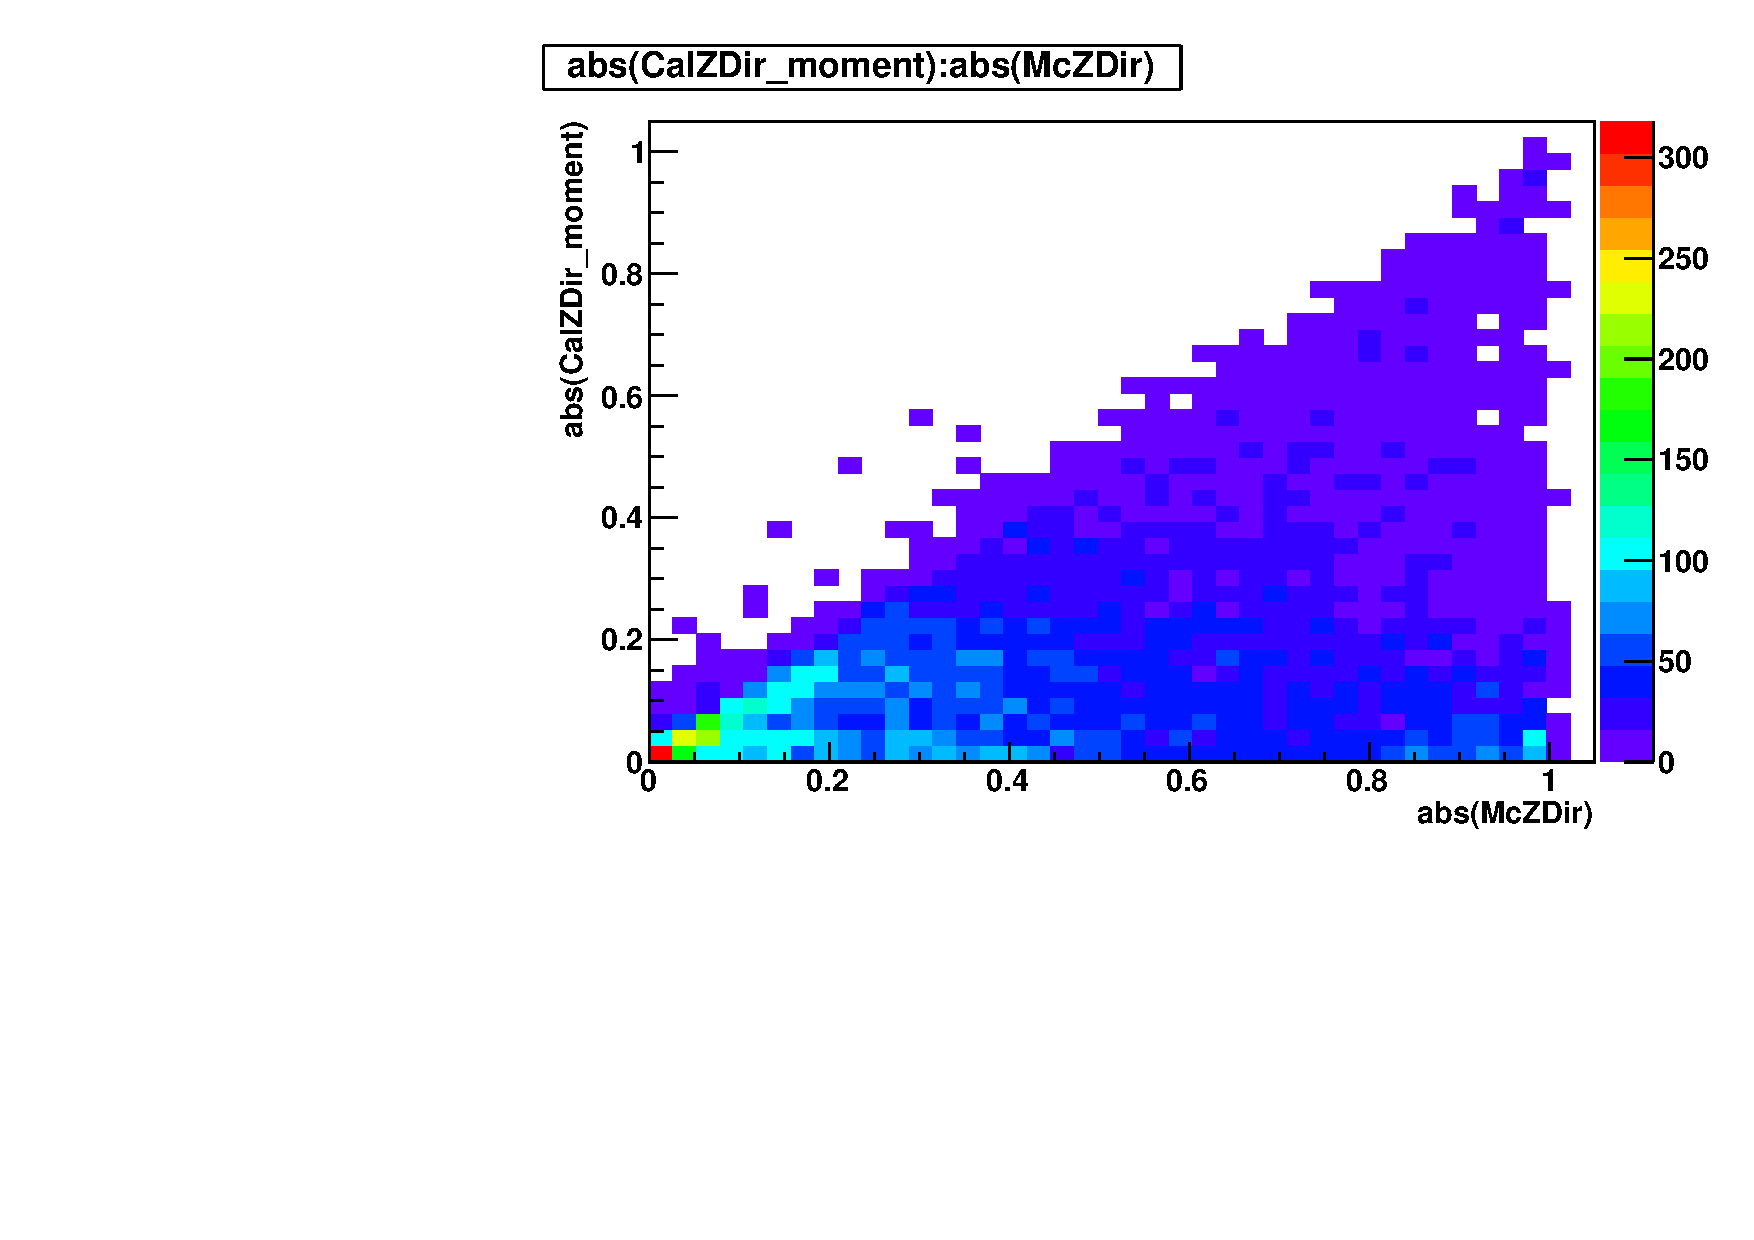
\includegraphics[width=0.6\textwidth]{McvsMoment}
  \end{center}
  \caption{The reconstructed direction (CalZDir-moment) vs true direction (McZDir).  }
  \label{McVsMoment}
\end{wrapfigure}

\begin{figure}[h!]
  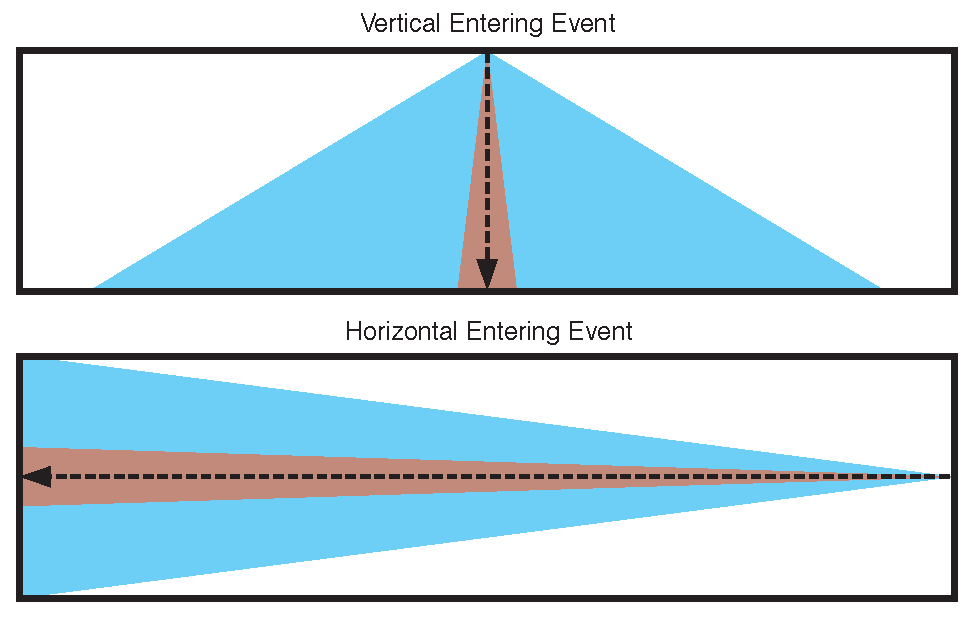
\includegraphics{showers.pdf}
  \caption{Cartoon examples of two hadronic showers, one vertical entering and one horizontal entering.  The black dotted line represents the track of the hadron.  The red shaded area is the leptonic core and the blue shaded area is the hadronic halo of the shower.}
  \label{showers}
\end{figure}

The above procedure is optimized for leptons and gamma-rays.  The problem is evident when one considers the differences between leptonic and hadronic showers.  Leptonic showers tend to small transverse shapes and deposit the entirety of the particle's incident energy into the shower.  This small transverse shape allows the moment analysis to correctly assume, even for relativity short path length events, that the longest axis corresponds to the particle's incident direction.  

Hadronic showers on the other hand contain a leptonic core but also a large hadronic halo.  This hadronic halo is populated by many low energy pion interactions.  The directional fitter may be affected by the hadronic halo since the hadronic halo is not necessarily symmetric in shape. This asymmetric halo shape can skew the position of the centroids in each layer causing the directional fitter to not return the incident angle.  The hadronic halo compounds problems for the moment analysis, remember that the moment analysis requires an input centroid and direction to trim the data and preform the iterative moment analysis, since the hadronic shower extends the size of the total shower.  We no longer have the case where the longest axis correlates to the incident direction of the charged particle.  This is especially true for vertical incident entering hadrons.  Since there is more material in the X-Y plane than Z direction the hadronic shower will have more material to interact with and produce a larger halo in the X-Y plane.  This can be seen in the cartoon examples in Figure \ref{showers}.  The moment analysis will falsely assign the direction to which every every transverse axis is longer as opposed to the correct longitudinal axis which correlates with direction of the hadron.  Conversely for horizontal entering events can traverse much more material along their incident direction and the hadronic halo tends to leak out the top and bottom  due to the CAL's rectangular shape.    We can see this affect in Figure \ref{McVsMoment}.  At McZDir $\sim$ 0 (horizontal incident) the direction reconstruction works well but at McZDir $\sim$ 1 (vertical incident) the direction reconstruction tends skew to horizontal directions.  

\subsection{Modified Moment Analysis}

The current state of reconstructing the direction for hadrons from the moment analysis is pretty bad.  The problem is the hadronic halo.  We want to modify the moment analysis to exclude the hadronic halo and focus the moment analysis on electromagnetic core and specifically the ionization track of the original hadron.  The ionization track is useful because it can additionally be used for particle identification.  

One way to filter out the hadronic halo is put a cut on the energy of the crystal used in the moment analysis.  Remember that pions, while numerous, tend to be much lower in energy than per hit than the energy deposited via ionization or nuclear interactions from the initial hadron or daughter spallation hadrons.  

The second idea is adjust the scaleFactor.  The scaleFactor is used to determine how hard isolated crystals are trimmed off of the data vector.    If the scaleFactor is too low too many crystals is initially trimmed from the data vector and the moment analysis will fail.  If the scaleFactor is too high then no isolated crystals will be dropped and the moment analysis will be skewed by these isolated crystals degrading the direction reconstruction.  We have to be careful about how to choose these two variables in order to optimize the modified moment analysis.  


\begin{figure}
        \centering
        \begin{subfigure}[b]{0.5\textwidth}
                \centering
                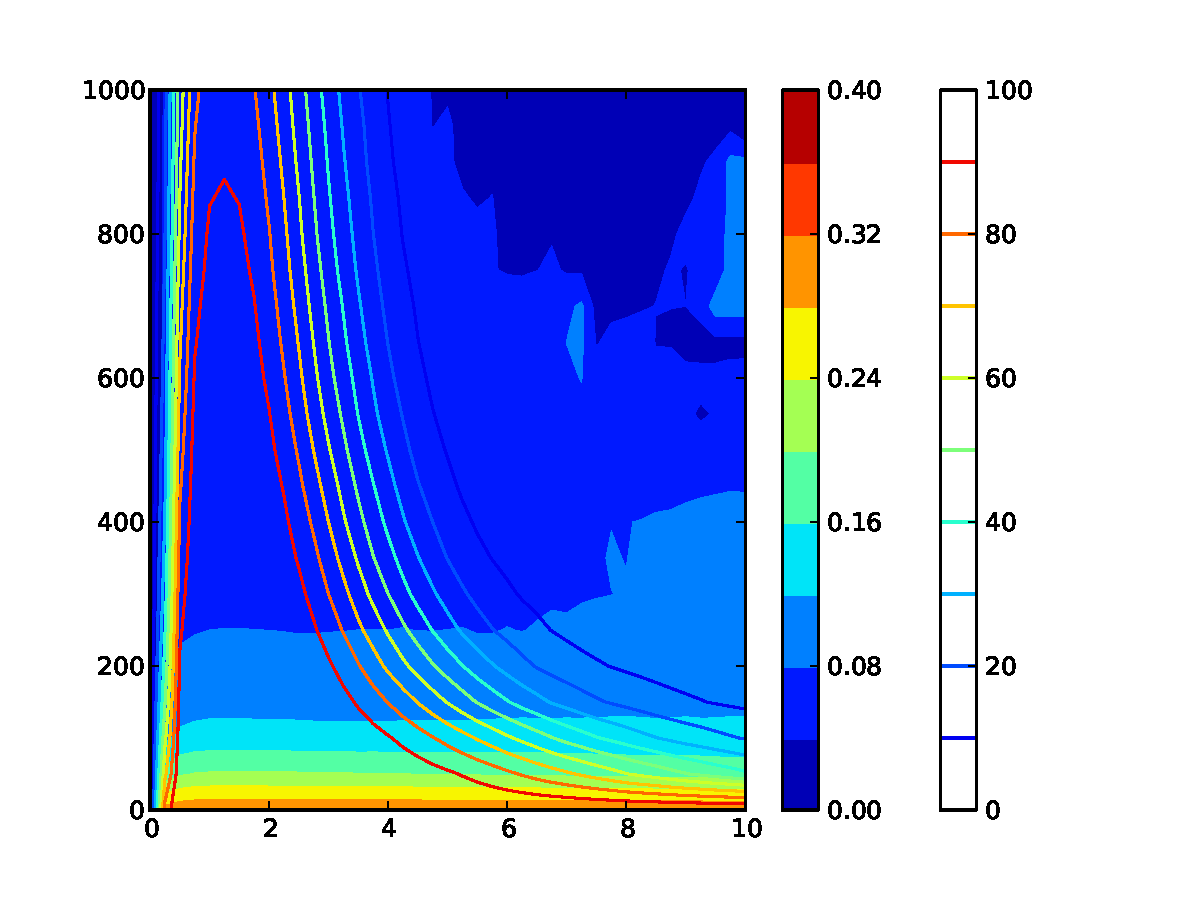
\includegraphics[width=\textwidth]{mean}
                \caption{The mean of the difference between CalZDir-moment and McZDir}
                \label{para_mean}
        \end{subfigure}%
        ~ %add desired spacing between images, e. g. ~, \quad, \qquad etc.
          %(or a blank line to force the subfigure onto a new line)
        \begin{subfigure}[b]{0.5\textwidth}
                \centering
                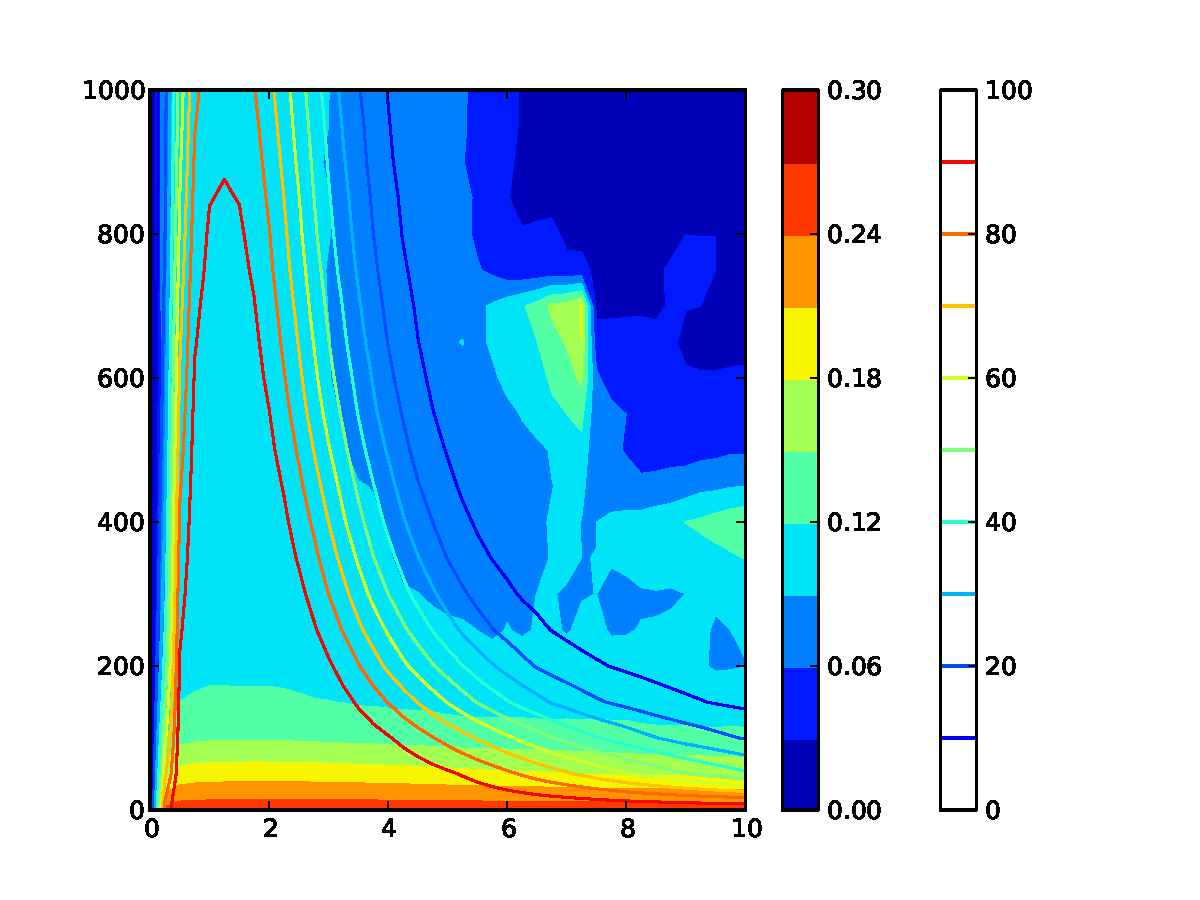
\includegraphics[width=\textwidth]{rms}
                \caption{The RMS of the difference between CalZDir-moment and McZDir}
                \label{para_rms}
        \end{subfigure}
        \caption{Exploring the parameter space between XtalCut and scaleFactor.  The color scale represents wither the mean or RMS of the difference between McZDir and CalZDir-moment.  The contours represent the success rate of the modified moment analysis.  }
        \label{para}
\end{figure}

The way we explore this parameter space is to vary both the crystal cut, called XtalCut from now on, and scaleFactor.  In Figure \ref{para_mean} and Figure \ref{para_rms}, I have varied both scaleFactor and XtalCut on the X and Y axis respectively and on the Z axis the either the mean difference between CalZDir-moment and McZDir or the RMS of the difference between CalZDir-moment and McZDir.  

We want a couple things from choosing the right scaleFactor and XtalCut. First we want the mean and RMS to be as low as possible.  That signifies that difference between McZDir and CalZDir-moment is small and the direction reconstruction has properly reconstructed the direction.  In addition we want a high success rate of the moment analysis.  Fortunately it appears by studying the phase space maps that the moment analysis is well behaved for both scaleFactor and XtalCut.

I nominally choose a scaleFactor of 1.5 and XtalCut of 400 MeV.

\subsection{Modified Directional Fitter}

I have also edited the directional fitter.  Unlike before where the directional fitter went first followed by the moment analysis I have reversed the process.  The reason is because the modified directional fitter requires an accurate direction and centroid position whereas the original directional fitter did not.  

The main difference between the original directional fitter and the modified directional fitter is the modified directional fitter does not have a top down bias.  The original directional fitter uses the energy centroid in each layer.  This restriction to each layers introduces a vertical entry bias into the directional fitter.  It will also poorly fit larger incident angle events since horizontal entering events and vertical entering events will look identical to the original fitter.  This will cause the original directional fitter to reconstruct horizontal entering events to vertical directions.  We modified to the directional fitter such that we break up the shower along the input direction from the modified moment analysis  into slices and find the position centroid in each of these slices.  We then fit the position of the centroids in X, Y, and Z to find the direction and the total centroid position.  We are also using the same XtalCut on the data vector for the modified directional fitter.  Since the modified directional fitter uses a a fitting algorithm we are also able to record the error in the direction and centroid position.  We can use this error information to filter out poor fits and further improve the PSF of the calorimeter for heavy ions.

\section{Results}

\begin{wrapfigure}{r}{0.6\textwidth}
  \begin{center}
    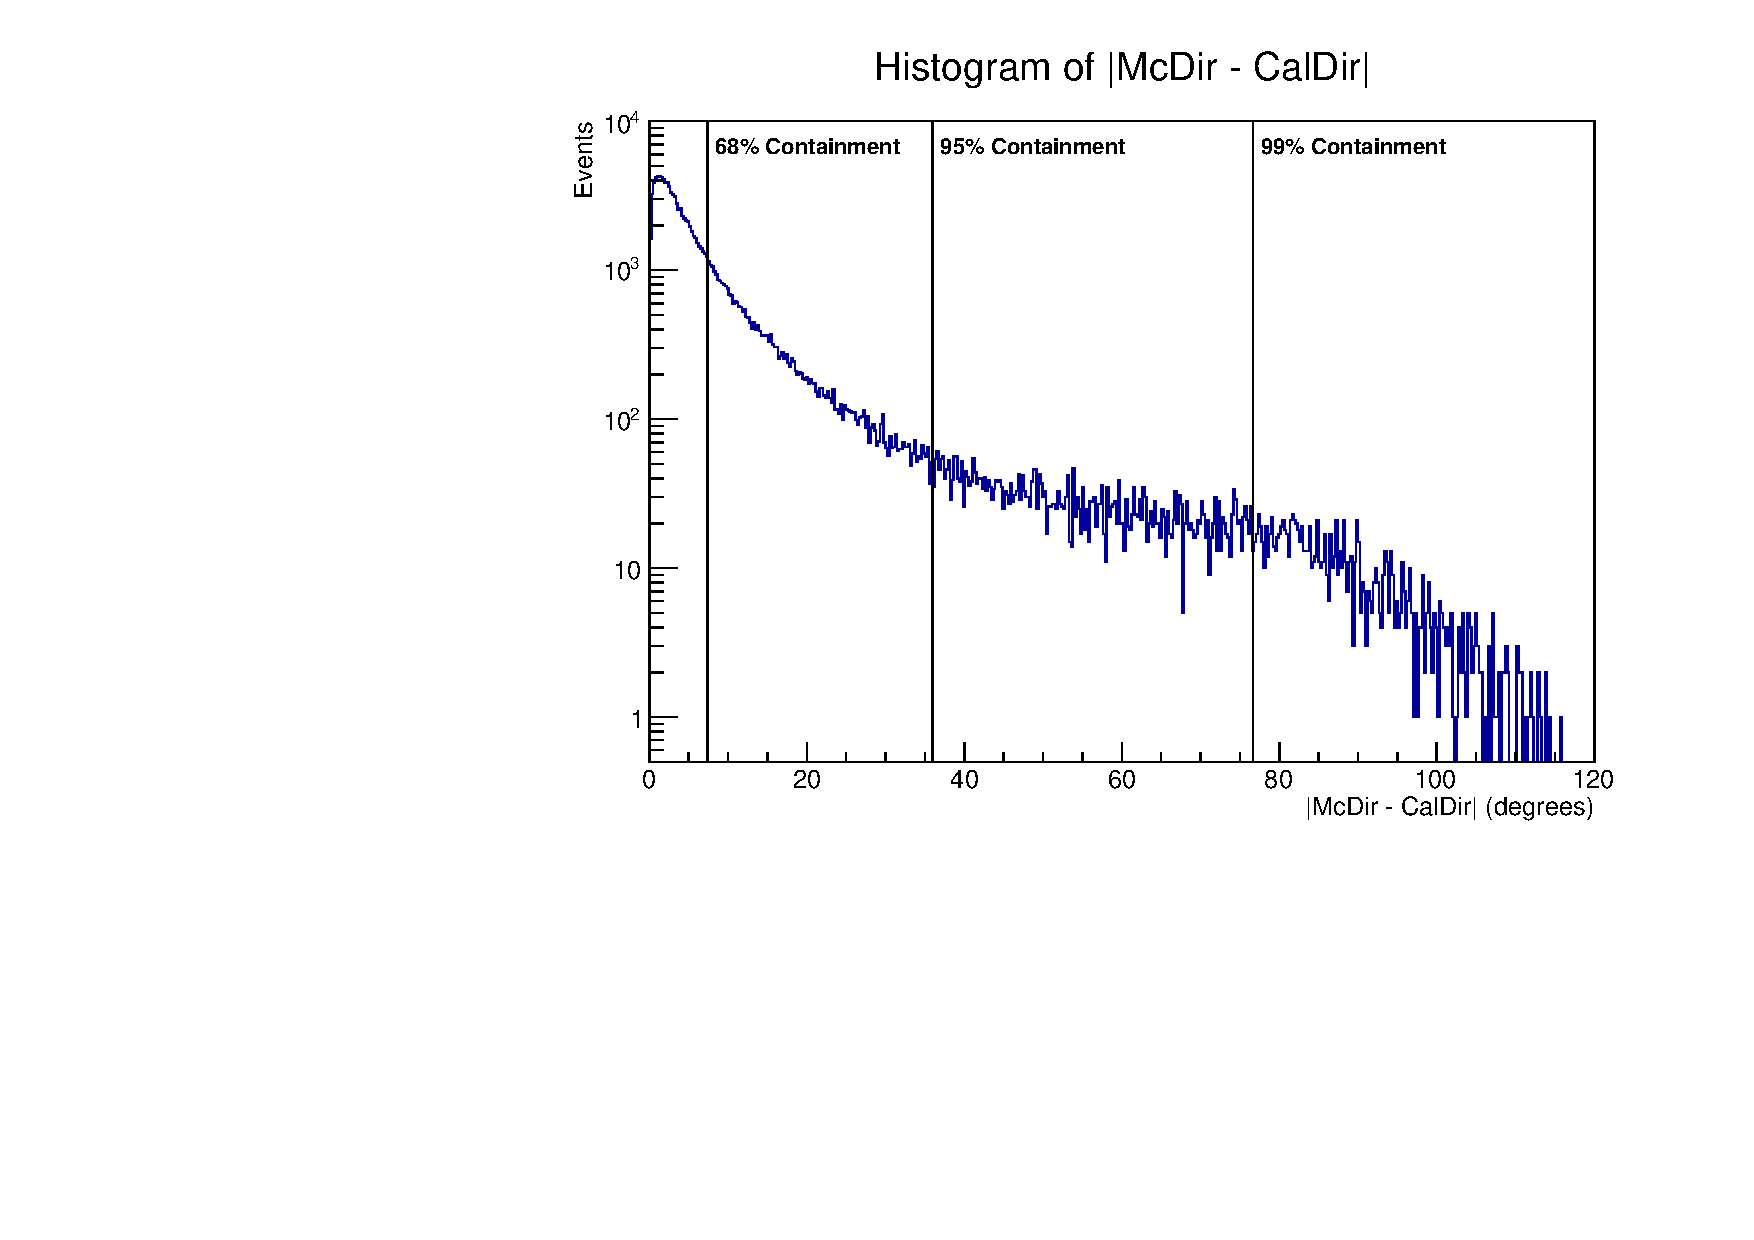
\includegraphics[width=0.6\textwidth]{psf}
  \end{center}
  \caption{Measuring different containment levels for reconstructed direction.  }
  \label{psf}
\end{wrapfigure}

How do these changes to the recon code improve out ability to measure the direction from heavy cosmic rays?  We have 4 scenarios:  the unmodified Pass7 recon, the modified pass 7 recon moment analysis, the modified pass 7 directional fitter analysis, and the Pass8 recon.  
I have calculated a rough PSF by taking the difference in the Monte Carlo direction and various reconstructed directions and integrating until 68\%, 95 \%, and 99 \% of the events have been summed.  We can see an example of how we measure the different containment percentages in \ref{psf}.

We now have a lot of plots to go over.  I found the different containment percentages for varying values of McEnergy (incident energy) and McZDir (incident angle) and for the different types of reconstructed direction.  The Monte Carlo used is a flat energy spectrum of boron and carbon coming from isotropic $4\pi$ Sr.  The version of GR used in the Pass7 and modified moment and directional analysis is GR-v17r35p3 and Pass8 is GR-20-09-04.


\newpage

Here is the set of plots for 68 \% containment for the various types of reconstruction directions:

\begin{figure}[h]
        \centering
        \begin{subfigure}[b]{0.5\textwidth}
                \centering
                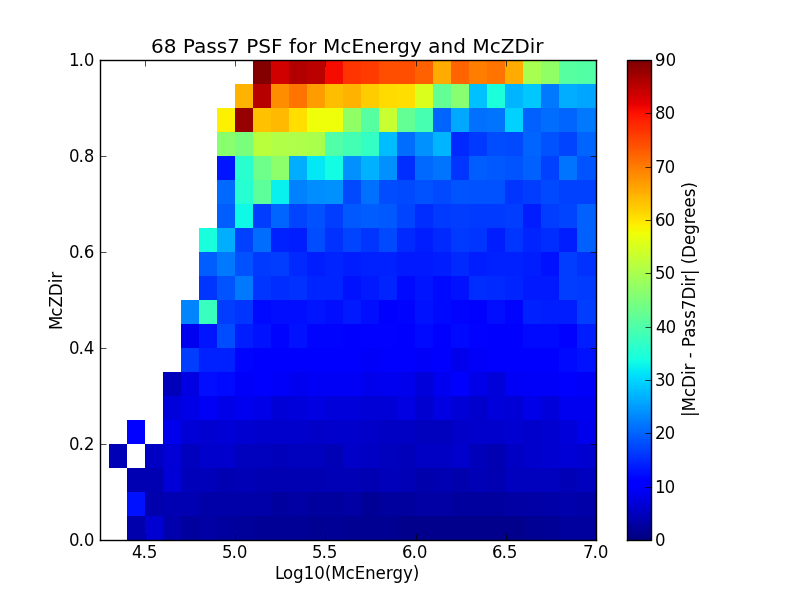
\includegraphics[width=\textwidth]{psf68_2D_pass7}
                \caption{68\% containment for Pass7}
                \label{con68_old}
        \end{subfigure}%
        \begin{subfigure}[b]{0.5\textwidth}
                \centering
                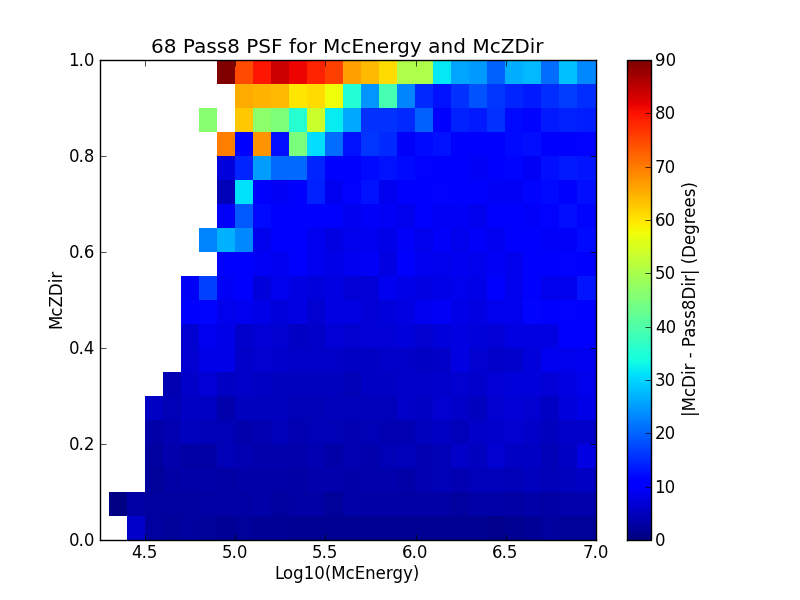
\includegraphics[width=\textwidth]{psf68_2D_pass8}
                \caption{68\% containment for Pass8}
                \label{con68_pass8}
        \end{subfigure}
                \begin{subfigure}[b]{0.5\textwidth}
                \centering
                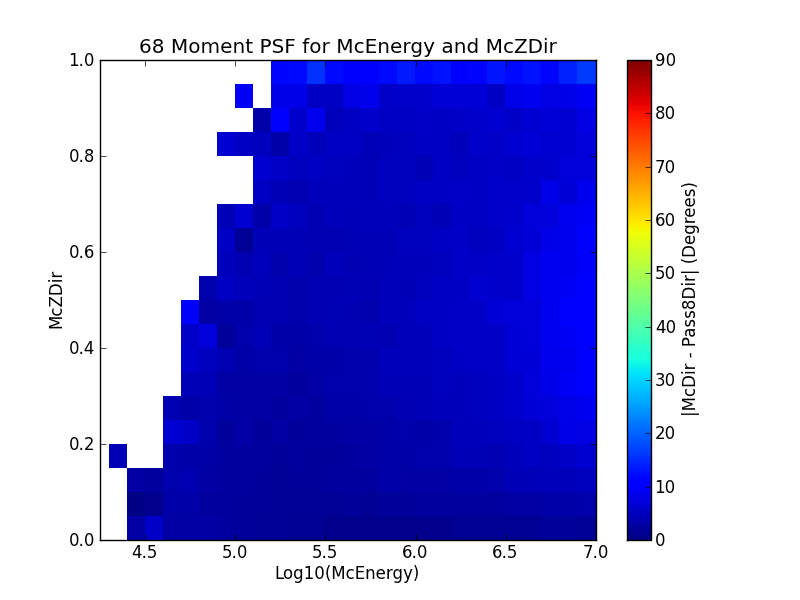
\includegraphics[width=\textwidth]{psf68_2D_moment}
                \caption{68\% containment for modified moment analysis}
                \label{con68_moment}
        \end{subfigure}%
        \begin{subfigure}[b]{0.5\textwidth}
                \centering
                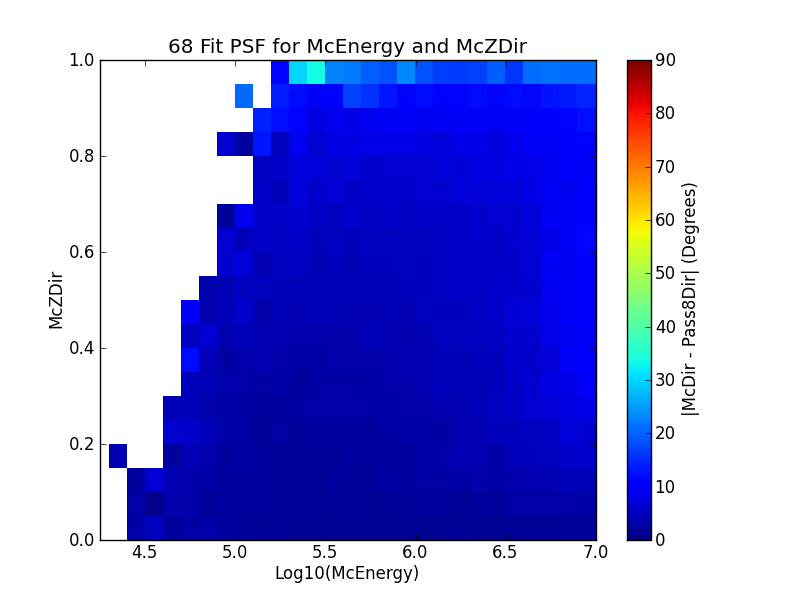
\includegraphics[width=\textwidth]{psf68_2D_fit}
                \caption{68\% containment for modified directional fitter}
                \label{con68_fit}
        \end{subfigure}
        \caption{The 68\% containment for McEnergy vs McZDir for the various different reconstructed directions }
        \label{con68}
\end{figure}

\newpage
Here is the set of plots for 95 \% containment for the various types of reconstruction directions:

\begin{figure}[h]
        \centering
        \begin{subfigure}[b]{0.5\textwidth}
                \centering
                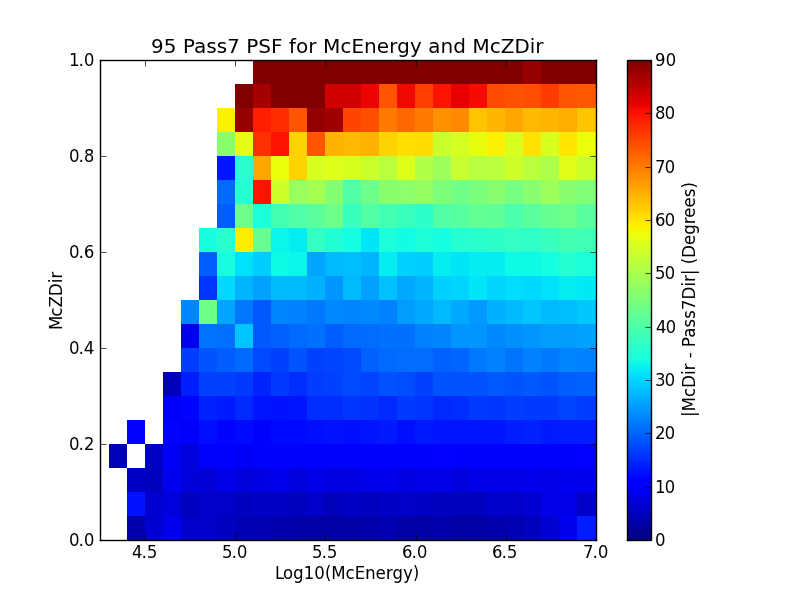
\includegraphics[width=\textwidth]{psf95_2D_pass7}
                \caption{95\% containment for Pass7}
                \label{con95_old}
        \end{subfigure}%
        \begin{subfigure}[b]{0.5\textwidth}
                \centering
                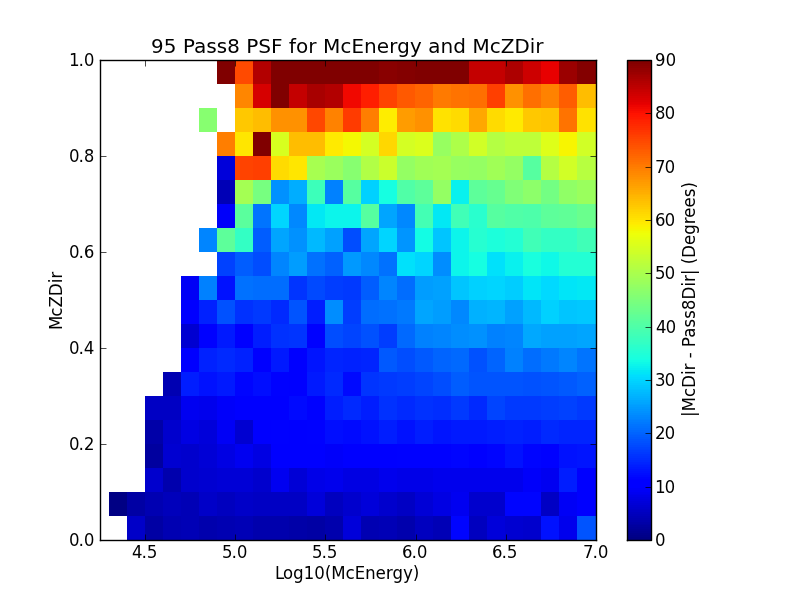
\includegraphics[width=\textwidth]{psf95_2D_pass8}
                \caption{95\% containment for Pass8}
                \label{con95_pass8}
        \end{subfigure}
                \begin{subfigure}[b]{0.5\textwidth}
                \centering
                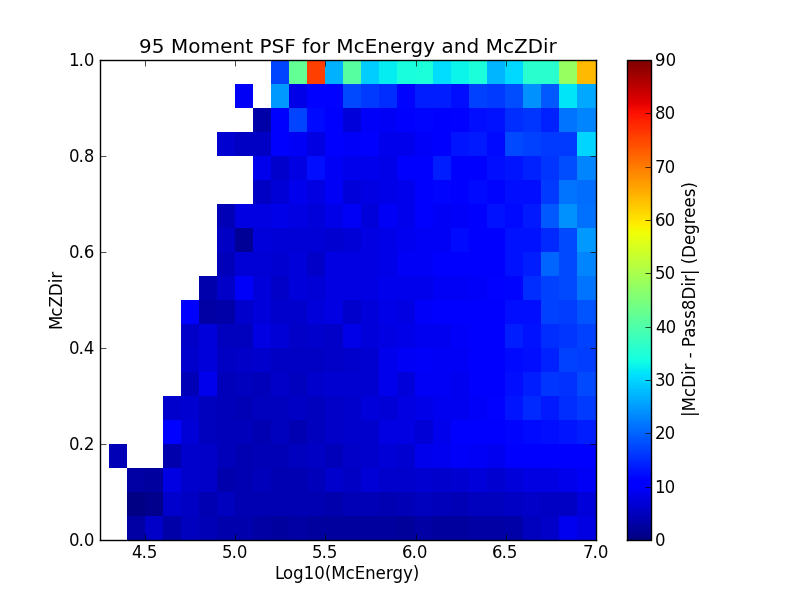
\includegraphics[width=\textwidth]{psf95_2D_moment}
                \caption{95\% containment for modified moment analysis}
                \label{con95_moment}
        \end{subfigure}%
        \begin{subfigure}[b]{0.5\textwidth}
                \centering
                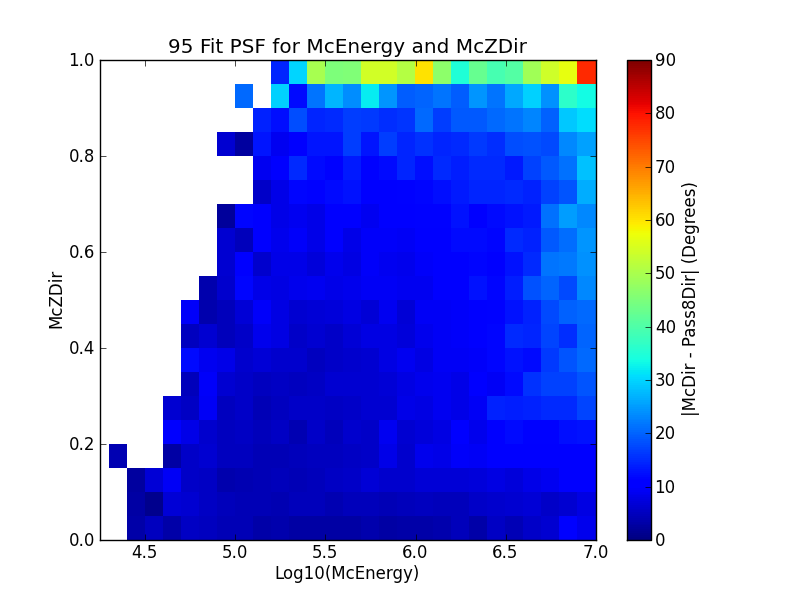
\includegraphics[width=\textwidth]{psf95_2D_fit}
                \caption{95\% containment for modified directional fitter}
                \label{con95_fit}
        \end{subfigure}
        \caption{The 95\% containment for McEnergy vs McZDir for the various different reconstructed directions }
        \label{con95}
\end{figure}

\newpage
Here is the set of plots for 99 \% containment for the various types of reconstruction directions:

\begin{figure}[h]
        \centering
        \begin{subfigure}[b]{0.5\textwidth}
                \centering
                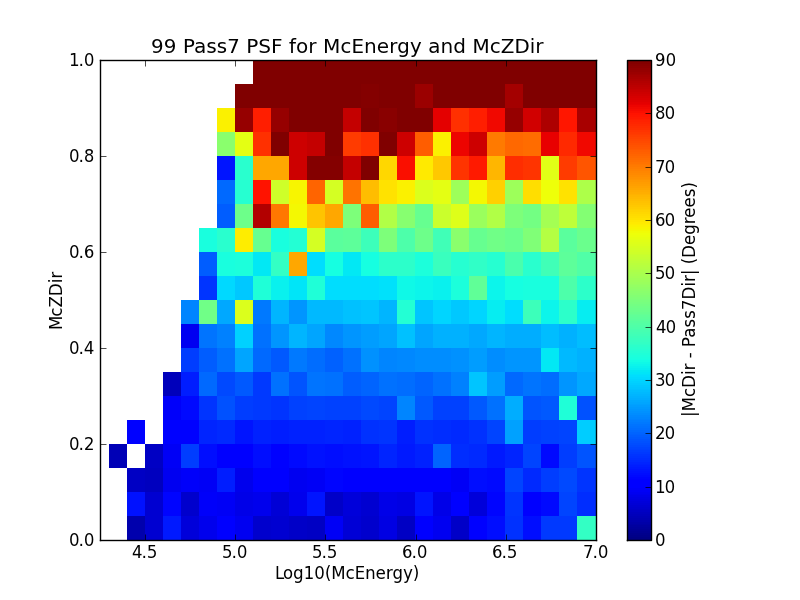
\includegraphics[width=\textwidth]{psf99_2D_pass7}
                \caption{99\% containment for Pass7}
                \label{con99_old}
        \end{subfigure}%
        \begin{subfigure}[b]{0.5\textwidth}
                \centering
                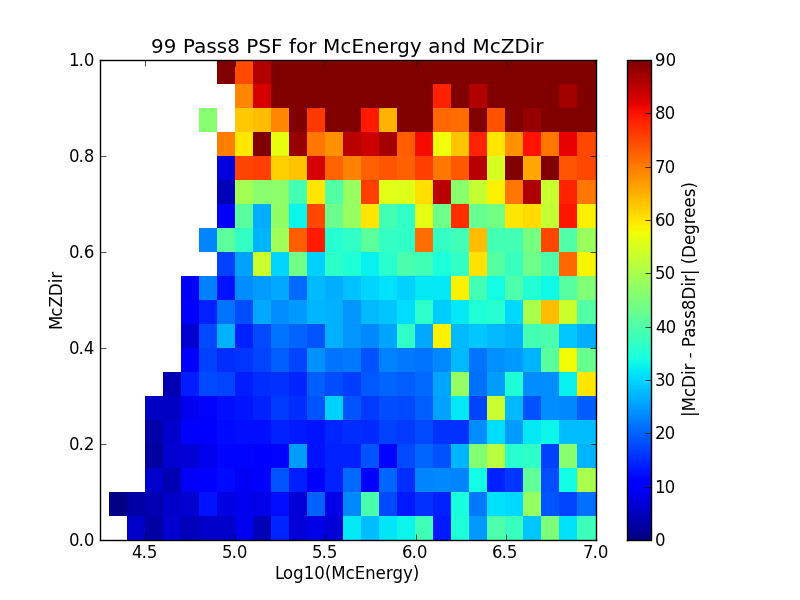
\includegraphics[width=\textwidth]{psf99_2D_pass8}
                \caption{99\% containment for Pass8}
                \label{con99_pass8}
        \end{subfigure}
                \begin{subfigure}[b]{0.5\textwidth}
                \centering
                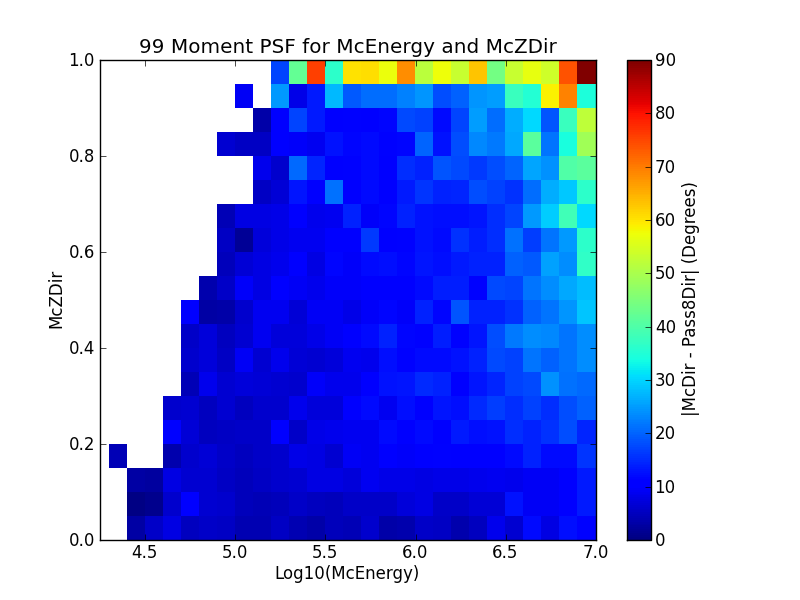
\includegraphics[width=\textwidth]{psf99_2D_moment}
                \caption{99\% containment for modified moment analysis}
                \label{con99_moment}
        \end{subfigure}%
        \begin{subfigure}[b]{0.5\textwidth}
                \centering
                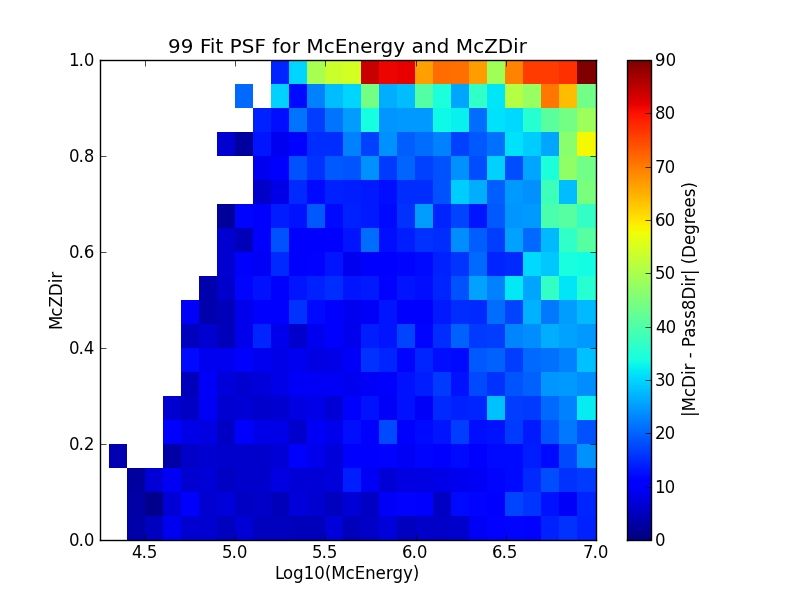
\includegraphics[width=\textwidth]{psf99_2D_fit}
                \caption{99\% containment for modified directional fitter}
                \label{con99_fit}
        \end{subfigure}
        \caption{The 99\% containment for McEnergy vs McZDir for the various different reconstructed directions }
        \label{con99}
\end{figure}

As we can see in the various containment percentages in Figures \ref{con68}, \ref{con95}, and \ref{con99};  that the modified moment analysis and the modified directional fitter are a vast improvement over either the Pass7 or Pass8 direction reconstruction for hadrons.  The hadron PSF for Pass7  and Pass8 are uniform with respect to McEnergy and McZDir.  The hadron PSF for the modified moment and directional fitter break down at near vertical incident angles and at very high incident energies.  Let's take a closer look at the $95\%$ containment by taking slices at specific energies and angles for the various types of direction reconstitution.  



\end{document}
